\begin{figure}[h]
  \centering

  \pgfplotsset{
    title style={font=\LARGE},
    label style={font=\LARGE},
    %ylabel style={rotate=-90},
  }
  \begin{tikzpicture}[scale=0.50]
    \begin{axis}[
      title=\textbf{Matrix Operation},
      xlabel=Block count ($\times10^3$ tasks),
      ylabel=Runtime (ms),
      legend pos=north west,
    ]
    \addplot+ [mark=*] table[x=X,y=Taskflow,col sep=space]{Fig/micro_benchmark/matrix_operation.csv};
    \addplot+ [mark=square] table[x=X,y=TBB,col sep=space]{Fig/micro_benchmark/matrix_operation.csv};
    \addplot+ [mark=+,color=magenta] table[x=X,y=OpenMP,col sep=space]{Fig/micro_benchmark/matrix_operation.csv};
    \legend{Cpp-Taskflow, TBB, OpenMP}
    \end{axis}
  \end{tikzpicture}
  %
  \begin{tikzpicture}[scale=0.50]
    \begin{axis}[
      title=\textbf{Graph Traversal},
      xlabel=Graph Size ($\times10^3$ tasks),
      ylabel=Runtime (ms),
      legend pos=north west,
    ]
    \addplot+ [mark=*] table[x=X,y=Taskflow,col sep=space]{Fig/micro_benchmark/graph_algorithm.csv};
    \addplot+ [mark=square] table[x=X,y=TBB,col sep=space]{Fig/micro_benchmark/graph_algorithm.csv};
    \addplot+ [mark=+,color=magenta] table[x=X,y=OpenMP,col sep=space]{Fig/micro_benchmark/graph_algorithm.csv};
    \legend{Cpp-Taskflow, TBB, OpenMP}
    \end{axis}
  \end{tikzpicture}
  %
  %\begin{tikzpicture}[scale=0.5]
  %  \begin{axis}[
  %    title=\textbf{Matrix Operation},
  %    xlabel=Number of CPUs,
  %    ylabel=Runtime (ms),
  %    legend pos=north west,
  %  ]
  %  \addplot+ [mark=*] table[x=X,y=Taskflow,col sep=space]{Fig/micro_benchmark/matrix_operation_speedup.csv};
  %  \addplot+ [mark=square] table[x=X,y=TBB,col sep=space]{Fig/micro_benchmark/matrix_operation_speedup.csv};
  %  \legend{Cpp-Taskflow, TBB}
  %  \end{axis}
  %\end{tikzpicture}
  %%
  %\begin{tikzpicture}[scale=0.5]
  %  \begin{axis}[
  %    title=\textbf{Graph Traversal},
  %    xlabel=Number of CPUs,
  %    ylabel=Runtime (ms),
  %    legend pos=north west,
  %  ]
  %  \addplot+ [mark=*] table[x=X,y=Taskflow,col sep=space]{Fig/micro_benchmark/graph_algorithm_speedup.csv};
  %  \addplot+ [mark=square] table[x=X,y=TBB,col sep=space]{Fig/micro_benchmark/graph_algorithm_speedup.csv};
  %  \legend{Cpp-Taskflow, TBB}
  %  \end{axis}
  %\end{tikzpicture}
  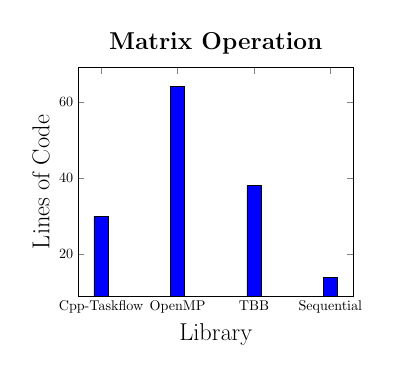
\begin{tikzpicture}[scale=0.51]
\begin{axis}[
    symbolic x coords={Cpp-Taskflow, OpenMP, TBB, Sequential},
    xtick=data,
    title=\textbf{Matrix Operation},
    xlabel=Library,
    ylabel=Lines of Code,
    ]
    \addplot[ybar,fill=blue] coordinates {
        (Cpp-Taskflow, 30)
        (TBB, 38)
        (OpenMP, 64)
        (Sequential, 14)
    };
\end{axis}
\end{tikzpicture}
  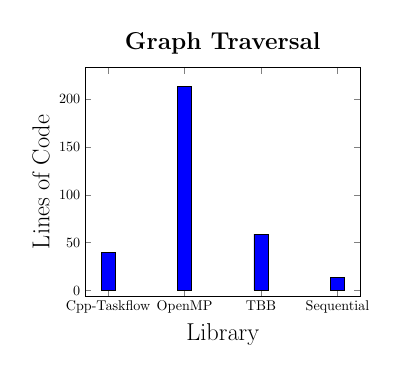
\begin{tikzpicture}[scale=0.51]
\begin{axis}[
    symbolic x coords={Cpp-Taskflow, OpenMP, TBB, Sequential},
    xtick=data,
    title=\textbf{Graph Traversal},
    xlabel=Library,
    ylabel=Lines of Code,
    ]
    \addplot[ybar,fill=blue] coordinates {
        (Cpp-Taskflow, 40)
        (TBB, 59)
        (OpenMP, 213)
        (Sequential, 14)
    };
\end{axis}
\end{tikzpicture}
  %\caption{Performance comparisons between Cpp-Taskflow, TBB, and OpenMP on two micro-benchmarks.}
  \label{fig::micro_benchmark}
\end{figure}

